% Created 2017-12-25 Mon 00:07
% Intended LaTeX compiler: pdflatex
\documentclass[11pt]{article}
\usepackage[utf8]{inputenc}
\usepackage[T1]{fontenc}
\usepackage{graphicx}
\usepackage{grffile}
\usepackage{longtable}
\usepackage{wrapfig}
\usepackage{rotating}
\usepackage[normalem]{ulem}
\usepackage{amsmath}
\usepackage{textcomp}
\usepackage{amssymb}
\usepackage{capt-of}
\usepackage{hyperref}
\usepackage{minted}
\usepackage{fancyhdr}
\setcounter{secnumdepth}{-1} 
\pagestyle{fancy}
\fancyhead{} 
\rhead{\textit{Michael Laufer}}
\lhead{\textit{Numerical Methods Fall 2017, HW6}}
\small

\author{mike}
\date{\today}
\title{}
\hypersetup{
 pdfauthor={mike},
 pdftitle={},
 pdfkeywords={},
 pdfsubject={},
 pdfcreator={Emacs 25.3.1 (Org mode 9.1.4)}, 
 pdflang={English}}
\begin{document}

\section{Advection-Diffusion Equation: FVM}
\label{sec:org40d2a12}
\subsection{Problem}
\label{sec:orgd0e4425}
Given the 1D advection-diffusion equation:
\[
\frac{d}{dx} \left( \rho u \phi - \Gamma \frac{d \phi}{dx} \right) = 0
\]
Subject to the boundary conditions:
\[
\phi(0) = 0, \phi(1) = 1
\]
Where \(\rho u\) is a constant.  \\
Using the definition of the Peclet number \(Pe = \frac{\rho u L}{\Gamma}\), the equation can be rearranged:
\[
\frac{d}{dx} \left( Pe \phi - \frac{d \phi}{dx} \right) = 0
\]

\subsection{Analytical Solution}
\label{sec:org2ea51fa}
The analytical solution is found by guessing a solution of the form 
\[
\phi =C_{1}e^{C_{2}x} +C_{3}$
\]
Plugging in and rearranging leads to:
\[
PeC_{1}C_{2}e^{C_{2}x} - C_{1}C_{2}e^{C_{2}x} = C_{1}C_{2}e^{C_{2}x}(Pe-C_{2))}=0
\] 
\[
\leadsto C_{2} = Pe
\]
Using boundary conditions:
\[
\phi (0) = C_{1} + C_{3} = 0 \leadsto C_{3} = -C_{1}
\] 
\[ 
\phi(1) = C_{1}e^{Pe}-C_{1} = 1 \leadsto C_{1} = \frac{1}{e^{Pe} -1} 
\]
Therefore:
\[ 
\phi(x) = \frac{1}{e^{Pe} -1} e^{Pex} - \frac{1}{e^{Pe} -1} 
\]
\subsection{Finite Volume Method}
\label{sec:org4d29ba2}
The Finite Volume Method (FVM) satisfies the governing equation on a finite-sized control volumes. The FVM enforces conservation laws which are based on the physics of the equation to be solved, leading to a "weak" of the equations, rather than the direct, "strong", form of the equation solved with the Finite Difference Method (FDM).

In the finite difference method the computational domain is split into \(n\) cells, where each cell has a cell center value and subsequent cell faces. The FDM is derived by integrating the governing equation over a finite control volume (cell). With the use of the fundamental theorem of calculus (in 1D) or Gauss's theorem (in multiple dimensions), the governing equation is reduced to a flux balance. In the case of the advection-diffusion equation:
\[
\left[ \rho u \phi - \Gamma \frac{d \phi}{dx} \right]_{e,i} - \left[ \rho u \phi - \Gamma \frac{d \phi}{dx} \right]_{w,i} = 0
\]
The question that remains is, how are values evaluated at the cell faces?
The simple approach is to use a central differencing approximation for the face values, effectively taking the mean of the adjacent cell-center values. For stability reasons, this is found to be unsuitable, particularly for the treatment of the advection term. In this assignment, we examine three alternate differencing schemes:

\begin{enumerate}
\item First-order Upwind Scheme
\item Second-order Upwind Scheme
\item QUICK Scheme
\end{enumerate}

\subsection{1st-Order Upwind Scheme}
\label{sec:org75214ca}
As opposed to the central differencing scheme, which takes the arithmetic mean of the adjacent cell center values to evaluate the cell face values, the upwind differencing evaluates a face value equal to the upstream cell-centered value. This is reasonable as due to the direction of the flow, the face value will be more affected by the upstream cell-centered value than the downstream value. 
Assuming a constant velocity, our problem reduces to:

\[
i=1: (12+3Pe \Delta x) \phi_{i} - 4 \phi_{i+1} = (8+3Pe \Delta x ) \phi_{L}} 
\] 
\[
i=2:,...,.N-1: (2+Pe \Delta x) \phi_{i} - \phi_{i+1} -(1+Pe \Delta x ) \phi_{i-1}} = 0
\]
\[
i=N: 12 \phi_{i} - (4 + 3 Pe \Delta x) \phi_{i-1} = (8-3Pe \Delta x ) \phi_{R}}
\]


The major disadvantage of this scheme compared to the central-differencing scheme is that it is only first order accurate (as opposed to second-order for the central differencing scheme.) Due to this limitation the second-order upwind scheme is developed.
\subsection{2nd-Order Upwind Scheme}
\label{sec:org8ff358f}
This scheme is similiar to the 1st-order version but effectively takes into account the cell centered values of \textbf{two} cells  in the upstream direction (as opposed to one). This makes the scheme second order accurate in space. For our problem, this reduces to:
\[
i=1: (12+6Pe \Delta x) \phi_{i} - 4 \phi_{i+1} = (8+6Pe \Delta x ) \phi_{L}} 
\] 
\[
i=2: (4+3Pe \Delta x) \phi_{i} - 2 \phi_{i+1} - (2 + 5 Pe \Delta x) \phi_{i-1} = -2Pe \Delta x \phi_{L}
\]  
\[
i=3:,...,.N-1: (4+3Pe \Delta x) \phi_{i} - 2\phi_{i+1} -(2 + 4 Pe \Delta x) \phi_{i-1} + Pe \Delta x \phi_{i-2} = 0
\]
\[
i=N: 24 \phi_{i} - (8 + 9 Pe \Delta x) \phi_{i-1} + (3 Pe \Delta x) \phi_{i-2} = (16-6Pe \Delta x ) \phi_{R}}
\]

This leads to a non-tridiagonal matrix which cannot be solved with the TDMA method. The Gaussian Elimination direct system of equation solver is employed to solve the system of linear equations.
\subsection{QUICK Scheme}
\label{sec:orgc3b83dd}
In the QUICK scheme, three cells are used to estimate the face value, one downstream, and two upstream, making this a nominally 3rd order accurate scheme. For out problem this reduces  to:

\[
i=1: (12+3Pe \Delta x) \phi_{i} + (Pe \Delta x -4) \phi_{i+1} = (8+4Pe \Delta x ) \phi_{L}} 
\] 
\[
i=2: (48+10Pe \Delta x) \phi_{i} + ( 9 Pe \Delta x -24) \phi_{i+1} - (24 + 27 Pe \Delta x) \phi_{i-1} = -8Pe \Delta x \phi_{L}
\]  
\[
i=3:,...,.N-1: (16+3Pe \Delta x) \phi_{i} + (3Pe \Delta x -8)\phi_{i+1} -(8 + 7 Pe \Delta x) \phi_{i-1} + Pe \Delta x \phi_{i-2} = 0
\]
\[
i=N: (96 - 9 Pe \Delta x) \phi_{i} - (32 + 18 Pe \Delta x) \phi_{i-1} + (3 Pe \Delta x) \phi_{i-2} = (64-24Pe \Delta x ) \phi_{R}}
\]

This also leads to a non-tridiagonal matrix which cannot be solved with the TDMA method. The Gaussian Elimination direct system of equation solver is again employed to solve the system of linear equations.

\subsection{Gaussian Elimination}
\label{sec:org3ff70c5}
Both the second-order upwind and QUICK schemes result in systems of equations that require a more generalized solver than the TDMA method. Gaussian Elimination involves two main steps, forward elimination, and backward substitution. The forward elimination step transforms the original coefficient matrix into an upper triangular matrix, where the last equation can be solved by just dividing the right hand side by the sole coefficient. Next, in the backward substitution step, the remaining unknowns are found by substituting just computed values into the equation just above. The method is illustrated in the following python code snippet:
\begin{minted}[]{python}
def gaussian(A, Q):
    # Forward Elimination
    K = len(Q)
    phi = np.zeros(len(Q))

    for k in range(K-1):
	for i in range(k+1,K):
	    const = A[i,k]/A[k,k]
	    for j in range(k+1,K):
		A[i,j] = A[i,j] - const*A[k,j]
	    A[i,k] = const
	    Q[i] = Q[i] -const*Q[k]

    # Backward Substitution
    phi[K-1] = Q[K-1]/A[K-1,K-1]
    for i in range(K-2,-1,-1):
	numerator = Q[i]
	for j in range(i+1, K):
	    numerator = numerator - A[i,j]*phi[j]
	phi[i] = numerator/A[i,i]
    return phi
\end{minted}
\subsection{Results}
\label{sec:org03d2b5e}
The problem is solved using all three schemes, where for each scheme, 20, 40, 80, and 160 cells are used along with 3 Peclet numbers. 0.1, 1.0 and 10.0 . In addition three different global Peclet numbers are examined: 0.1, 1, and 10. 
Solutions are plotted along with the respective error for each scheme on the same graph. 
\newpage
\subsubsection{Peclet = 0.1}
\label{sec:org47608ef}
\begin{center}
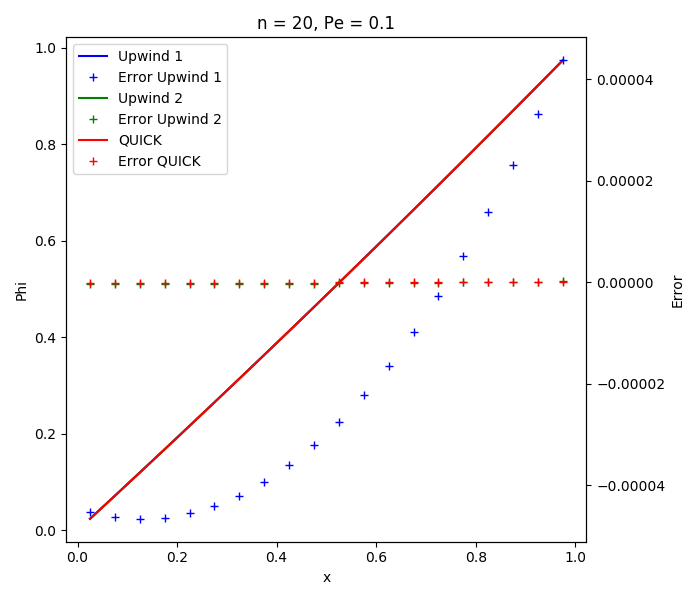
\includegraphics[width=10cm]{./figures/n20pe01.png}
\end{center}

\begin{center}
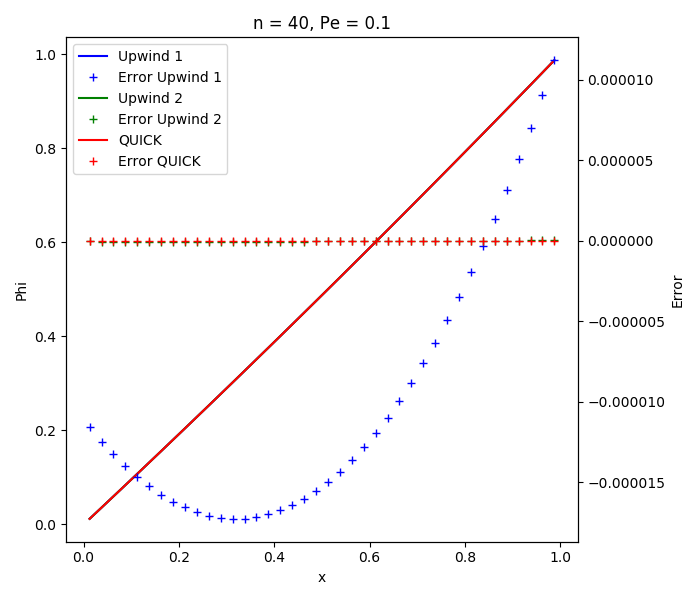
\includegraphics[width=10cm]{./figures/n40pe01.png}
\end{center}

\begin{center}
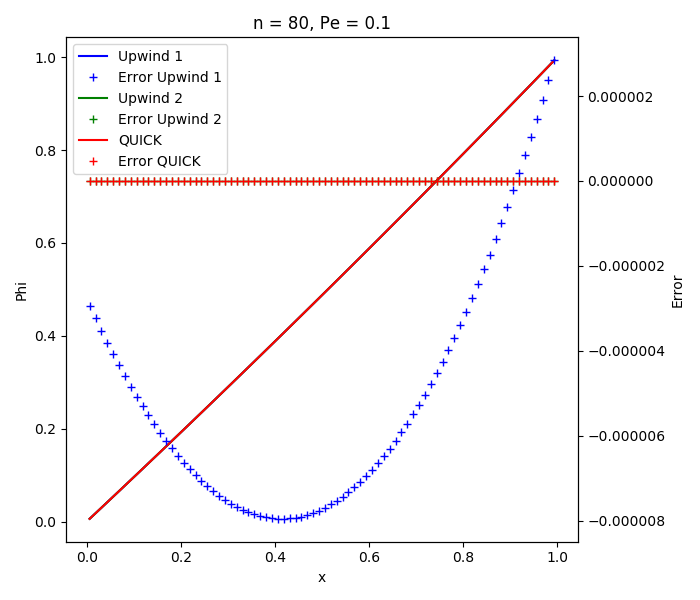
\includegraphics[width=10cm]{./figures/n80pe01.png}
\end{center}

\begin{center}
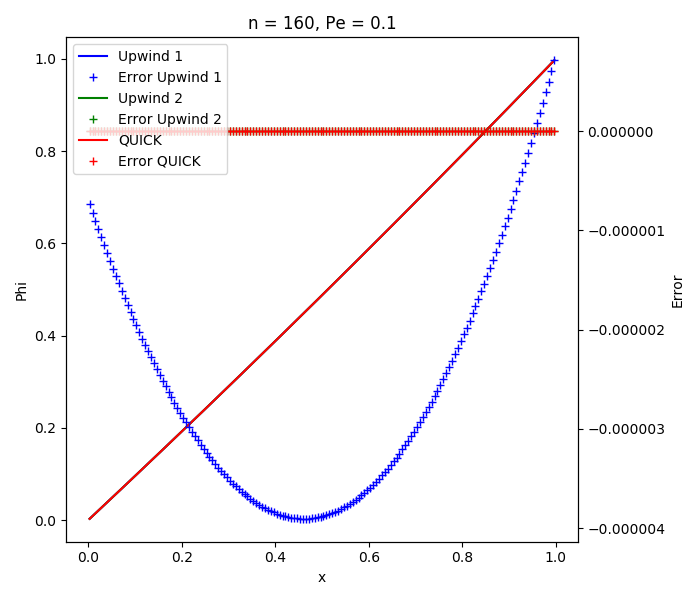
\includegraphics[width=10cm]{./figures/n160pe01.png}
\end{center}

\subsubsection{Peclet = 1.0}
\label{sec:orgcbebb65}
\begin{center}
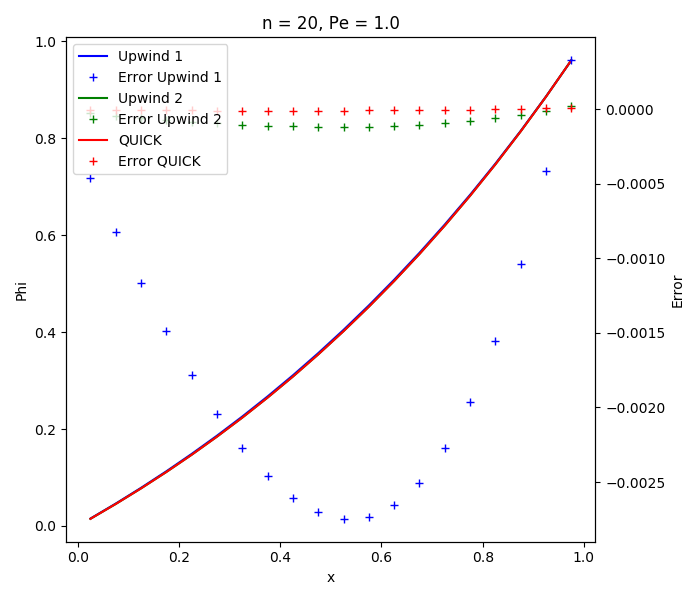
\includegraphics[width=10cm]{./figures/n20pe1.png}
\end{center}

\begin{center}
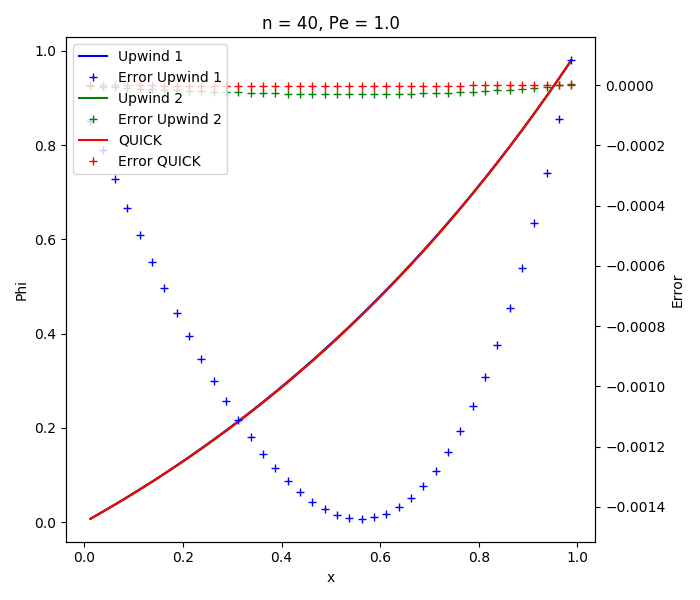
\includegraphics[width=10cm]{./figures/n40pe1.png}
\end{center}

\begin{center}
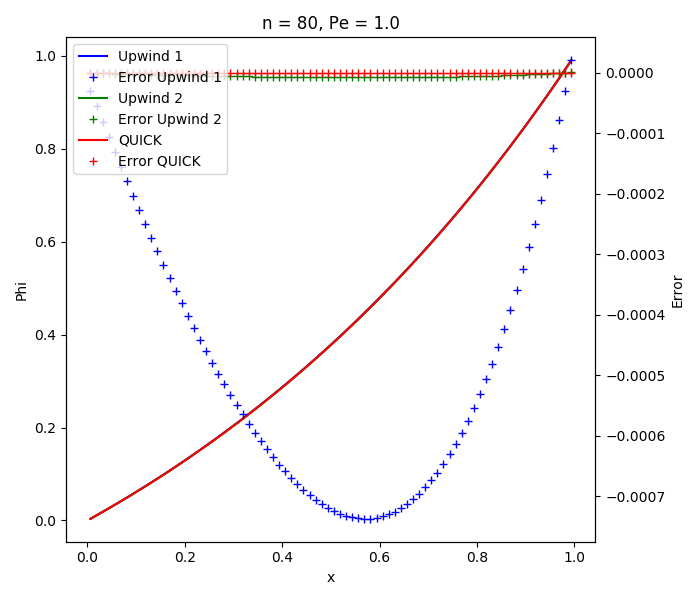
\includegraphics[width=10cm]{./figures/n80pe1.png}
\end{center}

\begin{center}
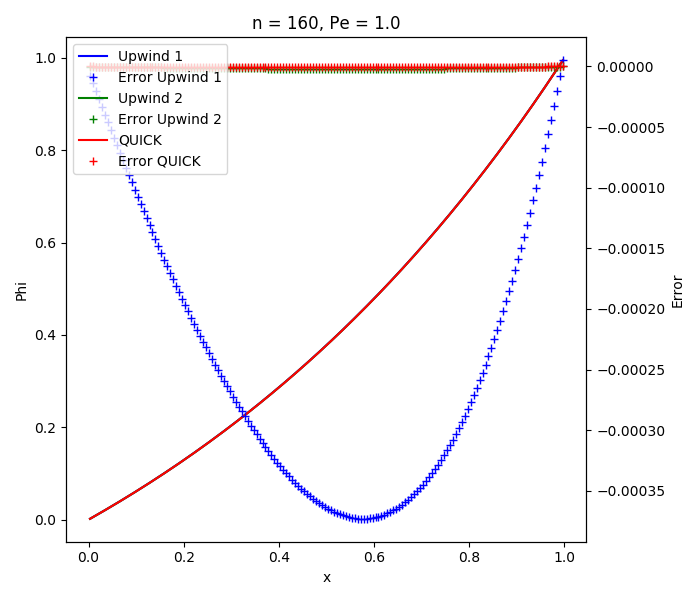
\includegraphics[width=10cm]{./figures/n160pe1.png}
\end{center}

\subsubsection{Peclet = 10.0}
\label{sec:orgca138ea}
\begin{center}
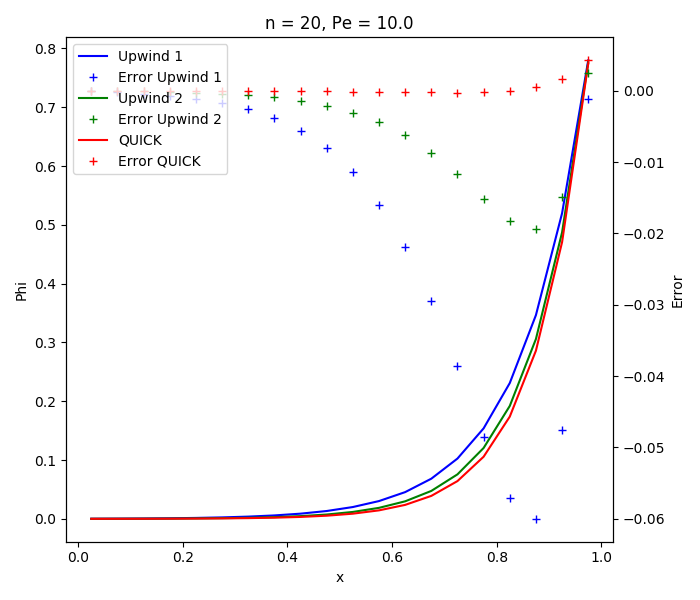
\includegraphics[width=10cm]{./figures/n20pe10.png}
\end{center}

\begin{center}
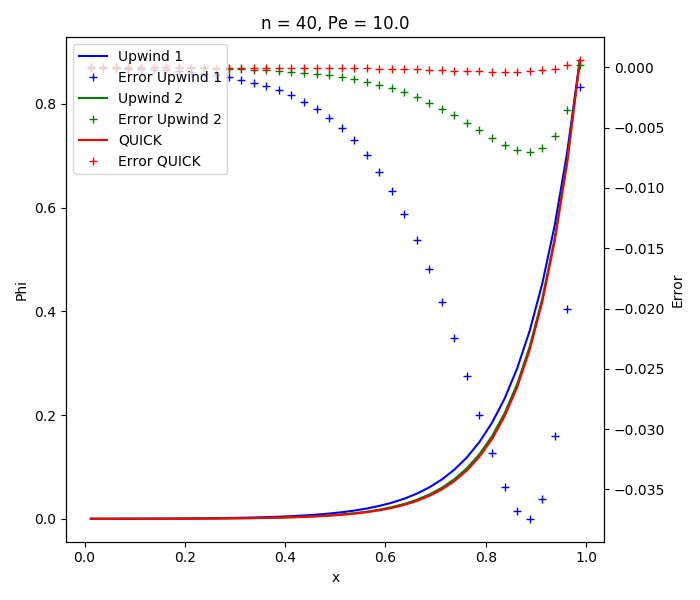
\includegraphics[width=10cm]{./figures/n40pe10.png}
\end{center}

\begin{center}
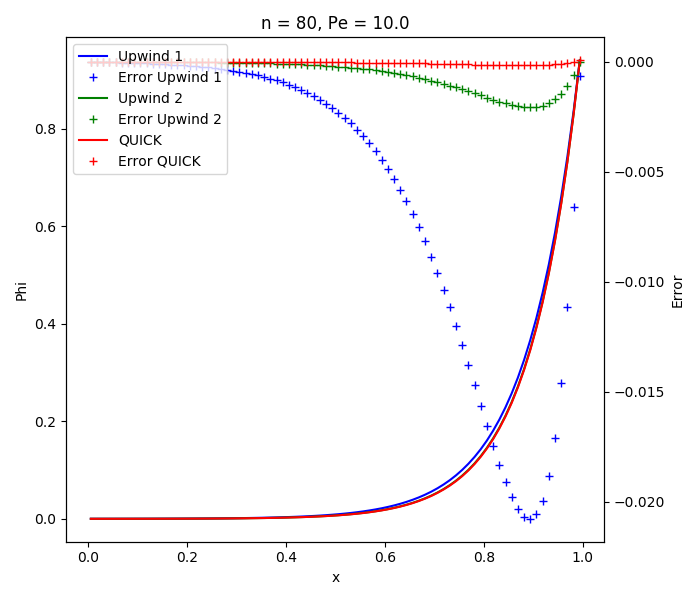
\includegraphics[width=10cm]{./figures/n80pe10.png}
\end{center}

\begin{center}
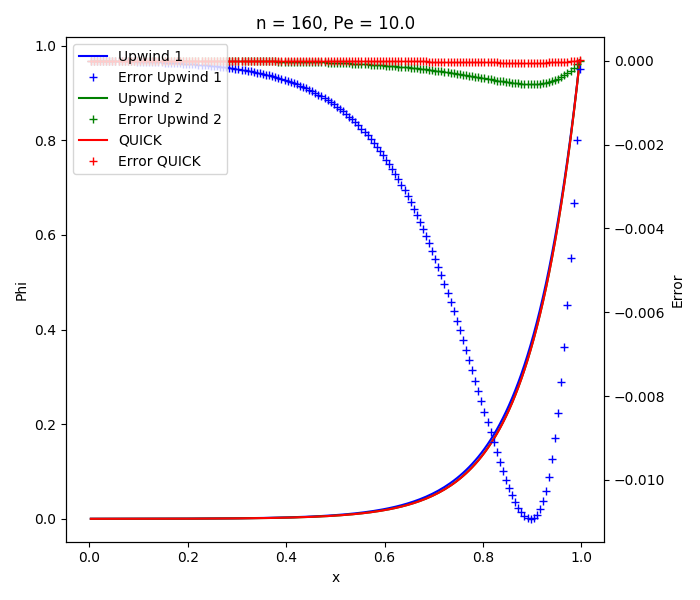
\includegraphics[width=10cm]{./figures/n160pe10.png}
\end{center}

\subsection{Discussion}
\label{sec:org3c31771}
Firstly we can notice that the errors are reduced as the number of nodes is increased. Moreover we observe that the 1st-order Upwind has much larger errors than the 2nd-order Upwind and the QUICK scheme. It is also noticeable that in general the QUICK scheme nets lower errors than the 2nd-order Upwind. This is due to the respective orders of the spatial error for each scheme, 1st, 2nd, and 3rd respectively. 

Additionally we notice that as the Peclet number is increased, the effect of advection becomes more pronounced, and the choice of the scheme becomes more critical. It is clear that one of the main advantages of the Finite Volume Method is the ability to choose how the flux at the face is evaluated depending on the physics of the problem, and required order of error. Upwinding methods such as the ones we have looked at in this exercise can allow for better stability of problems with high local Peclet numbers, while at the same time ensuring high levels of accuracy.  


\newpage
\section{Appendix: Python Code}
\label{sec:org63f96d8}
\begin{minted}[]{python}
import numpy as np
import matplotlib.pyplot as plt


def tridiag(A, Q):
    N = len(Q)
    ans = np.zeros(N)
    d = A.diagonal(0).copy()
    c = A.diagonal(1).copy()
    a = A.diagonal(-1).copy()
    Q = np.copy(Q)
    A = np.copy(A)

    for i in range(1,N):
	const = a[i-1]/d[i-1]
	d[i] = d[i] - const*c[i-1]
	Q[i] = Q[i] - const*Q[i-1]
    ans[N-1] = Q[N-1]/d[N-1]
    for i in range(N-2, -1, -1):
	ans[i] = (Q[i] -c[i]*ans[i+1])/d[i]
    return ans


def gaussian(A, Q):
    # Forward Elimination
    K = len(Q)
    phi = np.zeros(len(Q))

    for k in range(K-1):
	for i in range(k+1,K):
	    const = A[i,k]/A[k,k]
	    for j in range(k+1,K):
		A[i,j] = A[i,j] - const*A[k,j]
	    A[i,k] = const
	    Q[i] = Q[i] -const*Q[k]

    # Backward Substitution
    phi[K-1] = Q[K-1]/A[K-1,K-1]
    for i in range(K-2,-1,-1):
	numerator = Q[i]
	for j in range(i+1, K):
	    numerator = numerator - A[i,j]*phi[j]
	phi[i] = numerator/A[i,i]
    return phi



if __name__ == "__main__":
    title = "n = 20, Pe = 0.1"
    nx = 20 # 20, 40, 80, 160
    dx = 1.0 / nx
    x = np.linspace(0.0+ dx/2.0, 1-dx/2.0, nx)
    Pe = 0.1 # 0.1, 1.0, 10.0
    phi_L = 0.0
    phi_R = 1.0

    # Analytical solution
    phi_anal = (1.0/(np.exp(Pe)-1))*np.exp(Pe*x) - 1.0/(np.exp(Pe)-1) 

    # First-order upwind
    A = np.zeros((nx,nx))
    S = np.zeros(nx)
    for i in range(nx):
	if i == 0:
	    A[i,i] = (12 + 3*Pe*dx)
	    A[i,i+1] = -4.0
	    S[i] = (8 + 3*Pe*dx)*phi_L
	elif i == nx-1:
	    A[i,i] = 12.0
	    A[i,i-1] = -(4+3*Pe*dx)
	    S[i] = (8 -3*Pe*dx)*phi_R
	else:
	    A[i,i] = (2 + Pe*dx)
	    A[i,i+1] = -1.0
	    A[i,i-1] = -(1 + Pe*dx)
	    S[i] = 0.0
    phi_upwind_1 = tridiag(A,S)
    error_upwind_1 = phi_anal - phi_upwind_1

   # Second-order upwind
    A = np.zeros((nx,nx))
    S = np.zeros(nx)
    for i in range(nx):
	if i == 0:
	    A[i,i] = (12 + 6*Pe*dx)
	    A[i,i+1] = -4.0
	    S[i] = (8 + 6*Pe*dx)*phi_L
	elif i == 1:
	    A[i,i] = (4 + 3*Pe*dx)
	    A[i,i+1] = -2.0
	    A[i,i-1] = -(2+5*Pe*dx)
	    S[i] = -2*Pe*dx*phi_L
	elif i == nx-1:
	    A[i,i] = 24.0
	    A[i,i-1] = -(8+9*Pe*dx)
	    A[i,i-2] = 3*Pe*dx
	    S[i] = (16 -6*Pe*dx)*phi_R
	else:
	    A[i,i] = (4 + 3*Pe*dx)
	    A[i,i+1] = -2.0
	    A[i,i-1] = -(2 + 4*Pe*dx)
	    A[i,i-2] = Pe*dx
	    S[i] = 0.0
    phi_upwind_2 = gaussian(A,S)
    error_upwind_2 = phi_anal - phi_upwind_2

    # QUICK
    A = np.zeros((nx,nx))
    S = np.zeros(nx)
    for i in range(nx):
	if i == 0:
	    A[i,i] = (12 + 3*Pe*dx)
	    A[i,i+1] = (Pe*dx -4)
	    S[i] = (8 + 4*Pe*dx)*phi_L
	elif i == 1:
	    A[i,i] = (48 + 10*Pe*dx)
	    A[i,i+1] = (9*Pe*dx -24)
	    A[i,i-1] = -(24 + 27*Pe*dx)
	    S[i] = -8*Pe*dx*phi_L
	elif i == nx-1:
	    A[i,i] = (96 -9*Pe*dx)
	    A[i,i-1] = -(32 + 18*Pe*dx)
	    A[i,i-2] = 3*Pe*dx
	    S[i] = (64 -24*Pe*dx)*phi_R
	else:
	    A[i,i] = (16 + 3*Pe*dx)
	    A[i,i+1] = (3*Pe*dx -8)
	    A[i,i-1] = -(8 + 7*Pe*dx)
	    A[i,i-2] = Pe*dx
	    S[i] = 0.0
    phi_quick = gaussian(A,S)
    error_quick = phi_anal - phi_quick

    fig = plt.figure(figsize=(7,6))
    ax1 = fig.add_subplot(111)
    l1, l2, l3 = ax1.plot( x, phi_upwind_1, 'b', x, phi_upwind_2, 'g', x, phi_quick, 'r')
    ax1.set_ylabel("Phi")
    ax1.set_xlabel("x")

    ax2 = ax1.twinx()
    l4, l5, l6 = ax2.plot(x, error_upwind_1,'b+', x, error_upwind_2,'g+', x, error_quick, 'r+')
    ax2.set_ylabel("Error")
    fig.legend((l1, l4, l2, l5, l3, l6), ('Upwind 1', 'Error Upwind 1', 'Upwind 2', 'Error Upwind 2', 'QUICK', 'Error QUICK'), 'upper left', bbox_to_anchor=(0,1), bbox_transform=ax2.transAxes)
    plt.title(title)
    plt.tight_layout()
    plt.show()
\end{minted}
\end{document}